% ══════════════════════════════════════════════════════════════════════════════
%  SECTION – Problem Statement
% ══════════════════════════════════════════════════════════════════════════════

\section{Problem Statement}

Managing returnable transport items (RTIs) in a manufacturing supply chain is,
at its core, a closed-loop logistics problem. Raw materials, parts and finished goods flow in one direction, 
from suppliers to customers, but the RTIs that carry them must flow
back. The research question this paper addresses is the effectiveness of a collaborative return strategy of RTIs in a given SC, in which empty RTIs are rerouted and consolidated along the network, analyzing economic and environmental costs. To answer this, we propose an optimization model that determines the optimal return routes for empty RTIs,
the shipment frequency on each route, and the minimum RTI pool to prevent production disruptions, thereby defining the service network design for RTIs.

% ─────────────────────────────────────────────────────────────────
We model the SC as a directed graph $G = (V, E)$, where each node $i \in V$
represents a manufacturing site and each arc $(i,j) \in E$ represents a
potential transport route, both for empty and full RTIs. Figure \ref{fig:SC} illustrates a SC network,
where nodes are manufacturing sites and the black arcs represent the daily average flows of full
RTIs driven by production demand. Each product family requires a specific RTI
type, and the number of RTIs needed per shipment depends on how many raw materials, parts or finished goods fit
in a single RTI, as shown in Figure~\ref{fig:Product-RTI}.

\begin{figure}[h]
    \centering
        \resizebox{0.5\linewidth}{!}{\begin{tikzpicture}

  %% ── Supply-chain nodes ────────────────────────────────────────────────────
  \placeSCnodes

  %% ── Full RTI routes ───────────────────────────────────────────────────────
  \draw[routefull] (A) -- (B) node[midway, above, font=\scriptsize\bfseries]{10};
  \draw[routefull] (B) -- (C) node[midway, right, font=\scriptsize\bfseries]{15};
  \draw[routefull] (D) -- (A) node[midway, left,  font=\scriptsize\bfseries]{10};
  \draw[routefull] (E) -- (F) node[midway, right, font=\scriptsize\bfseries]{10};

%% ── Legend ────────────────────────────────────────────────────────────────
  \begin{scope}[shift={(\legendCoord)}]
    \node[scnode] (ln) at (0, 0) {};
    \node[right=0.1cm of ln, font=\scriptsize, text width=2.4cm] {SC nodes};
    
    \draw[routefull]  (-0.2, -0.6) -- (0.8, -0.6)
      node[right, font=\scriptsize] {Routes of full RTIs};
      
  \end{scope}
\end{tikzpicture}
}
    \caption{ Full RTIs routes }
    \label{fig:SC}
\end{figure}

\begin{figure}[h]
    \centering
        \resizebox{0.5\linewidth}{!}{

\begin{tikzpicture}[node distance=0.8cm and 0.5cm, font=\sffamily , perspective={
    p = {(0,0,0)}}]

% \begin{tikzpicture}[node distance=0.8cm and 0.5cm, font=\sffamily, tdplot_main_coords ]

  % Styles for boxes, ellipses, and colored labels



  % Gene nodes and numbers for container type 1
  \node[] (sw) {
\includegraphics[scale=0.1]{figures/003-steering-wheel.png}};

  
  \node[left= of sw] (w) {
\includegraphics[scale=0.1]{figures/004-motor.png}};
  \node[left= of w] (ce) {
\includegraphics[scale=0.1]{figures/006-car-engine.png}};
  \node[left= of ce] (cd) {
\includegraphics[scale=0.1]{figures/005-car-door.png}};
  \node[left= of cd] (s) {
\includegraphics[scale=0.1]{figures/007-seat.png}};
  \node[left= of s] (b) {
\includegraphics[scale=0.1]{figures/002-car.png}};

  \node[left= of b] (mt) {
\includegraphics[scale=0.1]{figures/001-manual-transmission.png}};


  \node[aux_gene_group, fit=(b) (mt)] (group1) {};
  

\node[below=1.5cm of group1] (box1) {\tikz     \drawblock{1}{1}{1}{\lbt}{\wbt}{\hbt}{red}{0}{0}{0};};
    \path [line] (b) -- node[midway, right] {$150$} (box1);
    \path [line] (mt) -- node[midway, left] {$10$} (box1);

  \node[aux_gene_group, fit=(ce) (s)] (group2) {};
  

\node[below=1.5cm of group2] (box2) {\tikz     \drawblock{2}{3}{5}{3}{1.5}{3}{blue}{0}{0}{0};};
    \path [line] (ce) -- node[midway, right] {$2$} (box2);
    \path [line] (s) -- node[midway, left] {$3$} (box2);
    \path [line] (cd) -- node[midway, left] {$4$} (box2);

  \node[aux_gene_group, fit=(sw) (w)] (group3) {};
  

\node[below=1.5cm of group3] (box3) {\tikz     \drawblock{2}{3}{5}{2}{1}{2}{purple}{0}{0}{0};};
    \path [line] (w) -- node[midway, right] {$5$} (box3);
    \path [line] (sw) -- node[midway, left] {$20$} (box3);



\end{tikzpicture}

}
    \caption{ Product quantities per RTI }
    \label{fig:Product-RTI}
\end{figure}

An RTI exists in one of two states: \textit{full}, when loaded with raw materials, parts and finished goods, or \textit{empty}, once its contents have been consumed at the
destination site. Some RTIs can be folded, reducing their volume to decrease transport costs, as shown in Figure~\ref{fig:stacked-rti}.
The simplest RTI return strategy is a one-to-one relationship, i.e., 
for every shipment of full RTIs a supplier sends to a customer, the customer
must return the empty RTIs along the same route, as depicted in
Figure \ref{fig:1to1RTI}. This strategy is operationally straightforward,
since each pair of nodes only coordinates with each other. However, it
is rarely cost-optimal in large SCs, as it ignores consolidation
opportunities along the SC and tends to result in both excessive empty RTI transport costs and a larger RTI pool than strictly necessary, which implies higher RTI investment and inventory costs.

\begin{figure}[ h ]
  \centering
  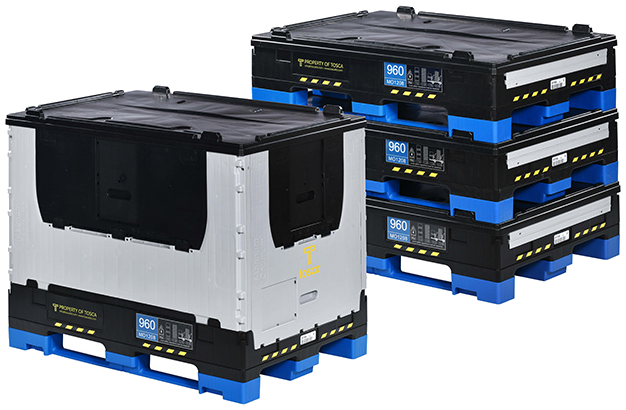
\includegraphics[width=0.4\linewidth]{figures/Magnum-Optimum_12108-removebg-preview.png}
  \caption{Full and empty folded RTIs}
  \label{fig:stacked-rti}
\end{figure}

\begin{figure}[h]
    \centering
        \resizebox{0.75\linewidth}{!}{\begin{tikzpicture}[
    % Define styles for consistent styling
    factory node/.style={
        circle,
        draw,
        minimum size=4.5cm,
        align=center,
        thick,
        fill=white
    },
    arrow/.style={
        -{Stealth[length=3mm, width=2mm]},
        thick
    },
    label text/.style={
        font=\sffamily,
        fill=white, % Adds a white background behind the text to break the line
        inner sep=4pt
    },
    plan text/.style={
        align=center, 
        font=\sffamily\small
    }
]

% -----------------------------------------
% 1. Main Circular Nodes (Plant & Supplier)
% -----------------------------------------
\node[factory node] (plant) at (0,0) {
    \includesvg[width=1.5cm]{figures/factory.svg}\\[0.3cm]
    Plant
};

\node[factory node] (supplier) at (14,0) {
    \includesvg[width=1.5cm]{figures/factory.svg}\\[0.3cm]
    Supplier
};

% -----------------------------------------
% 2. Curved Routing Arrows (Top & Bottom)
% -----------------------------------------
% Supplier -> Plant (Top)
\draw[arrow] (supplier) to[bend right=20] 
    node[label text] {Transport of full RTIs} (plant);

% Plant -> Supplier (Bottom)
\draw[arrow] (plant) to[bend right=20] 
    node[label text] {Transport of empty RTIs} (supplier);

% -----------------------------------------
% 3. Production Plan (Left side)
% -----------------------------------------
\node[plan text] (plan_left) at (-4, 0) {Production unloads \\ full RTIS};
% Arrows pointing to Plant
\draw[arrow] (plan_left.east) -- ($(plant.west)+(0, 0.6)$);
\draw[arrow] (plan_left.east) -- ($(plant.west)-(0, 0.6)$);

% -----------------------------------------
% 4. Production Plan (Right side)
% -----------------------------------------
\node[plan text] (plan_right) at (18, 0) {Production loads \\ empty RTIs};
% Arrows pointing to Supplier
\draw[arrow] (plan_right.west) -- ($(supplier.east)+(0, 0.6)$);
\draw[arrow] (plan_right.west) -- ($(supplier.east)-(0, 0.6)$);

\end{tikzpicture}
}
    \caption{ One-to-one RTI return strategy }
\label{fig:1to1RTI}
\end{figure}

When a central decision-maker, such as a dominant tier-1 manufacturer, an original equipment manufacturer (OEM) that owns the RTI pool, or a SC platform acting as manufacturing as a service (MaaS) {\color{red} Add reference}, has visibility over the entire network, a collaborative RTI return strategy becomes possible. Rather than using a one-to-one RTI return strategy, the model optimizes empty RTI routes, reducing the total distance an empty RTI journeys and consolidating routes. This simultaneously diminishes RTI return costs and the overall RTI pool size. Figure~\ref{fig:sc1to1} shows the one-to-one baseline, while Figure \ref{fig:scshared} illustrates how an optimized collaborative strategy reduces RTI return transport costs on the same network. Determining the service network design is the primary objective of this research.

\begin{figure}[H]
    \centering
    \begin{subfigure}[b]{0.49\linewidth}
        \centering
        \resizebox{\linewidth}{!}{\begin{tikzpicture}

  \placeSCnodes

  %% ── Full RTI routes (black) ───────────────────────────────────────────────
  \draw[routefull] (A) -- (B)
    node[midway, below=3pt, font=\scriptsize\bfseries]{10};
  \draw[routefull] (B) -- (C)
    node[midway, right=3pt, font=\scriptsize\bfseries]{15};
  \draw[routefull] (D) -- (A)
    node[midway, left=3pt,  font=\scriptsize\bfseries]{10};
  \draw[routefull] (E) -- (F)
    node[midway, right=3pt, font=\scriptsize\bfseries]{10};

  %% ── Empty RTI return routes (blue, slight offset) ─────────────────────────
  \draw[routeempty, transform canvas={yshift= 4pt}]
    (B) -- (A) node[midway, above=1pt, font=\scriptsize\bfseries, color=blue!70]{10};
  \draw[routeempty, transform canvas={xshift=-4pt}]
    (C) -- (B) node[midway, left=1pt,  font=\scriptsize\bfseries, color=blue!70]{15};
  \draw[routeempty, transform canvas={xshift= 4pt}]
    (A) -- (D) node[midway, right=1pt, font=\scriptsize\bfseries, color=blue!70]{10};
  \draw[routeempty, transform canvas={yshift= 4pt}]
    (F) -- (E) node[midway, above=1pt, font=\scriptsize\bfseries, color=blue!70]{10};

%% ── Legend ────────────────────────────────────────────────────────────────
  \begin{scope}[shift={(\legendCoord)}]
    \node[scnode] (ln) at (0, 0) {};
    \node[right=0.1cm of ln, font=\scriptsize, text width=2.4cm] {SC nodes};
    
    \draw[routefull]  (-0.2, -0.6) -- (0.8, -0.6)
      node[right, font=\scriptsize] {Routes of full RTIs};
      
    \draw[routeempty] (-0.2, -1.2) -- (0.8, -1.2)
      node[right, font=\scriptsize] {Return of empty RTIs};
  \end{scope}



\end{tikzpicture}
}
        \caption{\textit{One-to-one} relationship}
        \label{fig:sc1to1}
    \end{subfigure}
    \hfill
    \begin{subfigure}[b]{0.45\linewidth}
        \centering
        \resizebox{\linewidth}{!}{\begin{tikzpicture}

  \placeSCnodes

  %% ── Full RTI routes (black) ───────────────────────────────────────────────
  \draw[routefull] (A) -- (B)
    node[midway, above=2pt, font=\scriptsize\bfseries]{10};
  \draw[routefull] (B) -- (C)
    node[midway, right=3pt, font=\scriptsize\bfseries]{15};
  \draw[routefull] (D) -- (A)
    node[midway, left=3pt,  font=\scriptsize\bfseries]{10};
  \draw[routefull] (E) -- (F)
    node[midway, right=3pt, font=\scriptsize\bfseries]{10};

  %% ── Optimised empty-RTI return routes (blue) ──────────────────────────────
  % C sends 5 empties back up to B
  \draw[routeempty, transform canvas={xshift=-4pt}]
    (C) -- (B) node[midway, left=1pt, font=\scriptsize\bfseries, color=blue!70]{5};

  % C sends 10 empties sideways to E (shared consolidation)
  \draw[routeempty] (C) -- (E)
    node[midway, above=2pt, font=\scriptsize\bfseries, color=blue!70]{10};

  % D sends 10 empties up to A  (consolidated leg)
  \draw[routeempty, transform canvas={xshift=1pt}]
    (F) -- (D) node[midway, right, font=\scriptsize\bfseries, color=blue!70]{10};

%% ── Legend ────────────────────────────────────────────────────────────────
  \begin{scope}[shift={(\legendCoord)}]
    \node[scnode] (ln) at (0, 0) {};
    \node[right=0.1cm of ln, font=\scriptsize, text width=2.4cm] {SC nodes};
    
    \draw[routefull]  (-0.2, -0.6) -- (0.8, -0.6)
      node[right, font=\scriptsize] {Routes of full RTIs};
      
    \draw[routeempty] (-0.2, -1.2) -- (0.8, -1.2)
      node[right, font=\scriptsize] {Routes of empty RTIs};
  \end{scope}
\end{tikzpicture}



}
        \caption{SND with minimized RTI return transport cost}
        \label{fig:scshared}
    \end{subfigure}
    \caption{SND with minimized RTI return transport cost}
\end{figure}

On certain routes, full RTIs are accompanied by protective accessories,
such as nets or lids, that secure parts during transit. These
\textit{inlays} are themselves reusable and must be returned to the origin
site after unloading. Here the FTL and LTL, also known as groupage, transport modes are addressed. 

The model takes as input data the average daily flows of full RTIs between nodes, derived from released production plans over a planning horizon chosen by the decision-maker, typically a month, quarter, or year. These averages are assumed to be representative of the considered planning horizon, meaning that demands are sufficiently stable for the average to serve as reliable input data, without extreme imbalances that would render it misleading. 

{\color{blue}
While the physical routing of full RTIs is set in advance by established production and procurement contracts (i.e., a specific supplier must deliver to a specific customer a given set of products), the logistical execution of these forward flows is subject to optimization. Specifically, the model determines two operational parameters for the forward flows. First, it selects the optimal RTI type from a set of compatible options for each product. This selection affects the required transport capacity and the subsequent volume of empty returns, as different RTI types possess distinct dimensions and folding ratios. Second, the model determines the dispatch frequency for these full shipments. The shipment frequency governs the accumulation of inventory, creating a fundamental trade-off: longer intervals between shipments improve vehicle utilization and reduce fixed transport costs, but need a larger RTI pool to cover in-transit and waiting stock. Consequently, minimizing the total system cost requires the joint optimization of forward dispatch frequencies and packaging types, alongside the consolidation of empty return routes.
}

Under this assumption, the problem can be considered a service network design for RTIs, which consists of finding the tradeoff among daily RTI transport cost, which include transport costs for both full and empty RTIs; the inventory holding cost of the RTI pool; and CO$_2$ emissions from RTI transport. The model determines:

\begin{enumerate}
  \item Routes for empty RTI and inlay return flows.
  \item The RTI type selection for products with multiple compatible packaging options.
  \item The shipment frequency per route (both full and empty flows), expressed as a \textit{queue time} (Q-day), i.e.\ the number of days between consecutive dispatches.
  \item The transport mode per route, i.e. FTL or LTL.
  \item The total number of RTIs needed in the whole SC network.
\end{enumerate}

% ─────────────────────────────────────────────────────────────────
The problem encompasses a strategic-tactical decision level, using as input data the daily averages of RTI demand flows. In practice, the daily average flow of full RTIs between nodes is managed by medium-to-long-term production contracts and procurement agreements, which should remain stable over the planning horizon under consideration. The Q-days and transport modes are likewise set with a medium-to-long-term frequency rather than renegotiated daily or weekly. By optimizing strategic-tactical decisions for a given planning horizon, instead of multi-period decisions, the model is computationally efficient even for large industrial networks, where a fully operational multi-period optimization could be intractable to solve. Here, the strategic-tactical perspective provides a scalable upper bound on the achievable savings from collaborative RTI management, by establishing transport routes, Q-days and the RTI pool size, which can subsequently serve as input data for operational-level RTI transport planning.
